\styledchapter{Linear Regression}

\section{Basic Setup}

\begin{definition}	Suppose $(y,x,u)$ satisfy \[
		y = x' \beta + u; \quad \E(xu) = 0
	.\] 
	
	Suppose we have an iid sample $\{y_i, x_i\}_{i=1}^{n}$.
	
	Assume a unique ordinary least squares estimator exists: \[
		\hat{\beta} = \left( \frac{1}{n} \sum_{i=1}^{n} x_i x_i' \right)^{-1} \frac{1}{n} \sum_{i=1}^{n} x_i y_i
	.\] 
	
	In matrix notation: $Y = X\beta + U$ and $\hat{\beta} = (X'X)^{-1} X' Y$.
\end{definition}

\section{Finite Sample Inference}

\begin{assumption}[Linear conditional mean, homoskedasticity]	Suppose that $Y \mid X \sim N(X\beta, \sigma^2 I_n)$, so that \[
		Y = X\beta + U; \quad \E(U \mid X) = 0, \quad \operatorname{Var}(U \mid X) = \sigma^2 I_n
	.\] 
\end{assumption}

\begin{remark}	These assumptions (linear conditional mean, homoskedasticity) would be satisfied if the iid observations of $(y_i, x_i)$ are multivariate normal, which follows from normality of $(y_i,x_i)$ and independence across $i$. (The product of two marginal normal densities of independent RVs will be the joint density, but it coincides with the bivariate normal density with zero covariance).
	\begin{itemize}
		\item Joint normality of $(y,x)$ implies $\E(y \mid x) = x' \beta$ for some $\beta$ and $\operatorname{Var}(y \mid x)$ is constant.
		\item Independence of the $(y_i, x_i)$ from each other implies $(y_1, x_1', \ldots, y_n, x_n')'$ is multivariate normal.
		\item Hence, $Y \mid x_1, \ldots, x_n$ is multivariate normal (a property of conditional distributions of multivariate normals).
	\end{itemize}
\end{remark}

\begin{remark}	Another sufficient set of conditions is MLR.1-5 with normality:
	
	MLR.6: $y_i \mid x_i \sim N(x_i' \beta, \sigma^2)$.
	
	Together these assumptions imply: \[
		\hat{\beta}^{\text{OLS}} = (X'X)^{-1} X' Y \mid X \sim N(\beta, \sigma^2 (X'X)^{-1})
	.\] 
	This is because $Y \mid X \sim N(X\beta, \sigma^2 I_n)$, so we can premultiply by $\left( X'X \right)^{-1}X'$ and immediately get the result by scaling of a multivariate Gaussian variable.
\end{remark}

\begin{proposition}[Conditional distributions of $\hat{\beta}_j$ and $\hat{\sigma}^2$]
	Let $e_j$ be a $k \times 1$ column vector consisting of zeroes, except in position $j$, where there is a $1$.
	
	Then \[
		e_j' \hat{\beta} \mid X = \hat{\beta}_j \mid X \sim N(\beta_j, [\sigma^2 (X'X)^{-1}]_{j,j})
		,\] where the subscript $j,j$ indicates the $(j,j)$ entry of the associated matrix.\boxednote{This follows because \begin{align*}
		&\operatorname{Var}\left(\hat{\beta}_j \mid X\right) \\ &= \operatorname{Var}\left(e_j' \hat{\beta} \mid X\right)\\ &= e_j' \operatorname{Var}\left(\hat{\beta}\mid X\right) e_j
.\end{align*} }
	
	It turns out that \[
		\hat{\sigma}^2 = \frac{\text{SSR}}{n-k} \sim \frac{\sigma^2}{n-k} \cdot \chi^2_{n-k}
	.\] 
	This estimate is unbiased and consistent.\boxednote{To see why, consider that the vector of errors divided by $\sigma$, $\frac{U}{\sigma}$, is a column of independent $N(0,1)$ random variables. Taking the inner product of all $n$ coordinates yields a random variable that is $\chi^2_n$ distributed. We have \begin{align*}
				&\underbrace{\frac{U'U}{\sigma^2}}_{\sim \chi^2_n} \\
				&= \underbrace{\frac{U' P_X U}{\sigma^2}}_{\chi^2_k} \\
				&+ \underbrace{\frac{\overbrace{U'M_X U}^{\left( M_X U \right)'\left( M_X U \right)
				\hat{U}' \hat{U} = SSR}}{\sigma^2}}_{= \chi^2_{n-k}}
		.\end{align*} }
	\end{proposition}
	
\begin{proposition}[Exact $t$ statistic under normality; standard error]
	If $\sigma^2$ were known, we could write \[
			\frac{\hat{\beta}_j - \beta_j}{\sigma \sqrt{e_j' (X'X)^{-1} e_j}} \mid X \sim N(0,1)
		,\] though typically we must replace it with $\hat{\sigma}^2$, which yields: \[
			\frac{\hat{\beta}_j - \beta_j}{\hat{\sigma} \sqrt{e_j' (X'X)^{-1} e_j}} \mid X \sim t_{n-k}
		,\] because $\hat{\sigma}^2 = \frac{U' M_X U}{n-k}$ is independent\footnote{Conditional on $X$, $\hat{\beta}-\beta = (X'X)^{-1}X'U$ is a function of $P_XU$, while $\hat{\sigma}^2$ is a function of $M_XU$. Since $P_XM_X = 0$, these Gaussian vectors are uncorrelated conditional on $X$, hence independent.} of $\hat{\beta} - \beta$, conditional on $X$.\boxednote{A $t_\nu$ random variable can be written as $Z/\sqrt{W/\nu}$ where $Z \sim N(0,1)$, $W \sim \chi^2_\nu$, and $Z$ and $W$ are independent.}
		
		$\hat{\sigma} \sqrt{e_j' (X'X)^{-1} e_j}$ is called the standard error of $\hat{\beta}_j$, $\operatorname{se}(\hat{\beta}_j)$.
	\end{proposition}

\begin{remark}	Note that the expression on the left (conditional on $X$) is a pivot statistic, but not a statistic (since it involves the unknown quantity $\beta_j$). Once we make a hypothesis, we can get a statistic by replacing $\beta_j$ with $\beta_j^{0}$.
\end{remark}
\begin{remark}	To test $H_0: \beta_j = \beta_j^0$, we can form the $t$-statistic: \[
		T_n = \frac{\hat{\beta}_j - \beta_j^0}{\operatorname{se}(\hat{\beta}_j)}
	,\] which has a $t_{n-k}$ distribution under $H_0$.
	
	Let $t_{n-k,1-\alpha/2}$ be the $1 - \alpha/2$ quantile of the $t_{n-k}$ distribution. The test \[
		\varphi_n = \mathds{1}\left( |T_n| > t_{n-k,1-\alpha/2} \right)
	\] has rejection probability equal to $\alpha$ when $H_0$ is true, and rejection probability strictly greater than $\alpha$ when $H_0$ is false.
	
		Therefore $\varphi_n$ is of size $\alpha$.\footnote{Size is the $\sup$ of the probability of false rejection across all $\beta^{0}$ in the null parameter space. When $H_0: \beta = \beta^{0}$, then the null parameter space is a singleton, so the size equals the rejection probability at that single value.}
	\end{remark}

\begin{remark}[Formula for two-sided p-value]
	Let $F$ denote the CDF of $t_{n-k}$. Conditional on the data, the $p$-value is given by \[
		\hat{p}_n = \inf_{\alpha \in (0,1)} \left\{ |T_n| > t_{n-k,1-\alpha/2} \right\} = \inf_{\alpha \in (0,1)} \left\{ |T_n| > F^{-1}(1-\alpha/2) \right\}
	.\] 
	It is the smallest significance level at which the test rejects.
	
	Since $F^{-1}$ is strictly increasing and continuous, we obtain:\boxednote{Because \begin{align*}
			&\left| T_n \right| >  F^{-1}\left( 1- \frac{\alpha}{2} \right) \\ &\iff F\left( \left| T_n \right| \right) > 1 - \frac{\alpha}{2}
	\end{align*} and we can isolate $\alpha$.} \[
		\alpha = 2[1 - F(|T_n|)] = 2F(-|T_n|)
	,\] 
	where the second equality follows from symmetry of the $t$-distribution.
\end{remark}

\begin{remark}[One-sided alternatives]
	If we have information a priori on $\beta$ (for example, we know that a coin cannot be biased towards tails), then we can get increased power with a one sided test over a two sided test. The corresponding one-sided $p$-value is larger than the matching two-sided tail probability.
\end{remark}

\section{Large Sample Inference}

\begin{remark}	Joint normality allows us to obtain exact finite sample distributions for these statistics, but we may also appeal to asymptotic normality.
	
	Now suppose \[
		\sqrt{n}(\hat{\beta}_n - \beta) \xrightarrow{d} N(0, V)
	,\] where $V = \E(xx')^{-1} \E(u^2 xx') \E(xx')^{-1}$. Suppose also that $V$ is non-singular and $\hat{V}_n \xrightarrow{p} V$ is a consistent estimator of $V$.
\end{remark}
\begin{example}[Hypothesis testing with firms' production]
	To motivate the following proposition, consider firms producing according to \[
		Q(K,L) = A K^{\beta_1}L^{\beta_2} U
	\] for firm-specific productivity shock $U$. We wonder: Do firms in this industry exhibit CRS?

	Recalling that the comparison of $Q(rK,rL)$ to $rQ(K,L)$ determines return to scale, we take logs and want to write \[
		\ln{\left(Q_i\right)} = \underbrace{\ln{\left(A\right)}}_{\beta_0} + \beta_1 \ln{\left(K_i\right)} + \beta_2 \ln{\left(L_i\right)} + \underbrace{\ln{\left(U_i\right)}}_{V_i}
	.\] We specify a test with $\beta = \begin{bmatrix}
	\beta_0  \\
	\beta_1 \\ \beta_2
	\end{bmatrix}$ and the test $H_0: \begin{bmatrix}
	0 & 1 & 1
	\end{bmatrix} \beta = 1$ and $H_A: \begin{bmatrix}
	0 & 1 & 1
	\end{bmatrix}  \beta \ne 1$.
\end{example}

\begin{proposition}[Testing a single linear restriction]
	Consider testing \[
		H_0: r' \beta = c \quad \text{vs.} \quad H_1: r' \beta \ne c
	,\] where $r$ is some specified vector in $\R^{k+1}$, and $c$ is a scalar.
	
	By the CMT, we have $r' \left[ \sqrt{n} \left( \hat{\beta}- \beta \right) \right] \xrightarrow{d} r' N(0,V)$, so taking the $r'$ inside yields \[
		\sqrt{n}(r' \hat{\beta} - r' \beta) \xrightarrow{d} N(0, r' V r)
	,\] and so by Slutsky's theorem: \[
		\frac{\sqrt{n}(r' \hat{\beta} - r' \beta)}{\sqrt{r' \hat{V}_n r}} \xrightarrow{d} N(0,1)
	.\] The LHS is an asymptotic pivot, as the RHS does not depend the unknown $r' \beta$.
	
	Under $H_0$, we have $r'\beta = c$, so now the LHS is known (and thus a test statistic): \[
		T_n = \frac{\sqrt{n}(r' \hat{\beta}_n - c)}{\sqrt{r' \hat{V}_n r}} \xrightarrow{d} N(0,1)
	.\] 
	
	The test we use is $\varphi_n = \mathds{1}(|T_n| > z_{1-\alpha/2})$. It is of asymptotic size $\alpha$, because under $H_0$: \begin{align*}
		\P(\text{Reject } H_0) &= \P(|T_n| > z_{1-\alpha/2}) \\
		&= \P(T_n < -z_{1-\alpha/2}) + \P(T_n > z_{1-\alpha/2}) \\
		&\to \Phi(-z_{1-\alpha/2}) + 1 - \Phi(z_{1-\alpha/2}) \\
		&= \frac{\alpha}{2} + 1 - \left(1 - \frac{\alpha}{2}\right) \\
		&= \alpha
	,\end{align*}
	where the convergence follows from definition of $T_n$ converging in distribution to a $N(0,1)$ random variable.
	
	Use $\varphi_n = \mathds{1}(T_n > z_{1-\alpha})$ for testing $H_0: r' \beta \le c$ vs. $H_1: r' \beta > c$.

	\textbf{Developing a confidence set. }
	It follows by definition of convergence in distribution that for any value of $r' \beta$: \[
		\lim_{n \to \infty} \P_{r' \beta} \left( \left| \frac{\sqrt{n}(r' \hat{\beta} - r' \beta)}{\sqrt{r' \hat{V}_n r}} \right| \le z_{1-\alpha/2} \right) = 1 - \alpha
	.\] 
	
	Since $z_{\alpha/2} = -z_{1-\alpha/2}$ by symmetry of the standard normal about $0$, rearranging to find the values of $r'\beta$ such that the test statistic is less than $z_{1-\frac{\alpha}{2}}$ in magnitude yields that \[
		C_n = \left[ r' \hat{\beta} - z_{1-\alpha/2} \sqrt{\frac{r' \hat{V}_n r}{n}}, \, r' \hat{\beta} + z_{1-\alpha/2} \sqrt{\frac{r' \hat{V}_n r}{n}} \right]
	\] is an asymptotic $1 - \alpha$ confidence interval for $r' \beta$.\boxednote{Note that it makes sense to talk about the \emph{probability} of $r'\beta \in C_n$ despite $r'\beta$ being a constant because $C_n$ is a random set.}
\end{proposition}

\begin{proposition}[Testing Multiple Linear Restrictions]
	Suppose we have the production function \[
		Q(K_i, L_i, \mu_i) = A K_i^{\beta_1} L_i^{\beta_2} \mu_i^{\beta_3} U_{i}
	.\] What if we want to test \[
		H_0: \beta_3 = 0, \quad \beta_1 + \beta_2 +\beta_3 = 1
	?\] 
	We can do this by writing multiple linear restrictions: \[
		R \beta =
		\begin{bmatrix}
			0 & 0 & 0 & 1 \\
			0 & 1 & 1 & 1
		\end{bmatrix} \begin{bmatrix}
		\beta_0 \\
		\beta_1 \\ \beta_2 \\ \beta_3
		\end{bmatrix} = \begin{bmatrix}
		0 \\
		1
		\end{bmatrix} 
	.\] 

	In general, we consider testing \[
		H_0: R\beta = c \quad \text{vs.} \quad R\beta \ne c
	,\] where $R$ is a $p \times k$-dimensional matrix of full row rank and $c$ is a $p \times 1$ vector.
	
	The full rank condition means none of our restrictions are redundant.
	
	By the CMT, we have $R \left( \sqrt{n} \left( \hat{\beta}- \beta \right) \right) \xrightarrow{d} R N(0,V)$, so bringing $R$ inside yields \[
		\sqrt{n}(R\hat{\beta}_n - R\beta) \xrightarrow{d} N(0, RVR')
	,\] where $RVR'$ is full rank (because $R$ and $V$ are), and hence positive definite (because $V$ is). We note that we do not know what $RVR'$ is because the variance is unknown.
	
	To see that $RVR'$ is positive definite, note that if $a \ne 0$, $R' a \ne 0$, so \[
		(R' a)' V(R' a) > 0
	,\] because $V$ is positive definite.
	
	A positive definite and symmetric matrix $A$ has a square root $A^{1/2}$ with inverse $A^{-1/2} = (A^{-1})^{1/2}$.
	
		Because $\left( R \hat{V}_n R' \right)^{-\frac{1}{2}} \xrightarrow{p} \left( R V_n R' \right)^{-\frac{1}{2}}$, we get from Slutsky's theorem and eliminate the problem of not knowing the asymptotic variance $RVR'$ with \[
			(R\hat{V}_n R')^{-1/2} \sqrt{n}(R\hat{\beta}_n - R\beta) \xrightarrow{d} N(0, I_p)
		.\] 
	
		\boxednote{For intuition, if $R\hat{\beta}$ is far from $c = R \beta$ in the Euclidean norm in $\R^p$, then the inner product of $R \hat{\beta} - c$ with itself should be large.} Inner producting the LHS ($\in \R^p$) with itself yields\footnote{The multivariate normality of the original random variable in $\R^p$ implies that the transformed coordinates are jointly normal. We use the CMT to get that the inner product with itself is the sum of $p$ independent $N(0,1)$ random variables, which is a $\chi^2_p$ random variable.} \[
		n \cdot (R\hat{\beta}_n - R\beta)' (R\hat{V}_n R')^{-1} (R\hat{\beta}_n - R\beta) \xrightarrow{d} \chi^2_p
	.\] 
	
	Under $H_0$, \[
		T_n = n \cdot (R\hat{\beta}_n - c)' (R\hat{V}_n R')^{-1} (R\hat{\beta}_n - c) \xrightarrow{d} \chi^2_p
	,\] and so we reject iff $T_n > \chi^2_{p,1-\alpha}$.
\end{proposition}

\begin{proposition}[Asymptotic Confidence Set for $R\beta$]
		There are generally two ways to find an asymptotic confidence set:
		\begin{enumerate}[label=(\roman*)]
			\item Test inversion: solving for $r' \beta$
			\item Acceptance region method: $r' \beta$ lies in the confidence set if the test statistic computed using $r' \beta$ does not exceed the critical value. In other words, given a value, we can conduct the test; if the test statistic is below the critical value, then the value would be in the confidence set.
				This is particularly useful when inverting the test statistic (in $r'\beta$) is difficult.
		\end{enumerate}

	Our example is well-suited to this second approach due to difficulty in inverting the test statistic.
	We simply define \[
		C_n = \left\{ c \in \R^p : n \cdot (R\hat{\beta} - c)' (R\hat{V}_n R')^{-1} (R\hat{\beta} - c) \le \chi^2_{p,1-\alpha} \right\}
	\] is an asymptotic $1 - \alpha$ confidence set for $R\beta$.
	
	This set is an ellipsoid centered at $R\hat{\beta}$, and satisfies \[
		\P_{R\beta}(R\beta \in C_n) \to 1 - \alpha
	.\] 
	
		Taking $R = I_k$ yields an asymptotic $1 - \alpha$ confidence set for $\beta$ (we essentially conduct $k$ tests on each of the individual components).
	\end{proposition}

\section{Heteroskedasticity}

Recall that \[
	\operatorname{Var}\left(\hat{\beta}^{OLS} \mid X\right) = \left( X'X \right)^{-1}X' \Omega X \left( X'X \right)^{-1}
,\] where \[
	\Omega = \operatorname{diag}\left( \E\left[u_1^2 \mid X_1\right] ,\ldots,\E\left[u_n^2 \mid X_n\right]  \right)
.\] This yields \[
	\operatorname{Var}\left(\hat{\beta}^{OLS} \mid X\right) = \left( \sum x_i x_i' \right)^{-1} \sum \E\left[u_i ^2 \mid x_i\right] x_i x_i ' \left( \sum x_i x_i' \right)^{-1}
.\]\boxednote{
	The robust variance uses the sandwich form with $\hat{\Omega}=\operatorname{diag}(\hat{u}_1^2,\ldots,\hat{u}_n^2)$.
} 
Earlier, we replaced $\E\left[u_i^2 \mid X_i\right] $ with $\hat{u}_i^2$ to form $\widehat{\operatorname{Var}(\hat{\beta}^{OLS}\mid X)}$.

In the univariate case, we had that \[
	\operatorname{Var}\left(\hat{\beta}_1\right) = \frac{\sigma^2}{\sum \left( x_i - \overline{x} \right)^2}
,\] so \[
	se(\hat{\beta}_1) = \sqrt{\frac{\hat{\sigma}^2}{\sum \left( x_i - \overline{x} \right)^2}} 
.\] The heteroskedasticity-robust standard error is \[
	se_{\text{rob}}(\hat{\beta}_1) = \sqrt{\frac{\sum \hat{u}_i^2 \left( x_i - \overline{x} \right)^2}{\sum\left( x_i - \overline{x} \right)^2}} 
.\] 

This expression makes sense. Consider the following data distribution:
\begin{figure}[htpb]
	\centering
	\caption{Benefits of robust standard errors}
	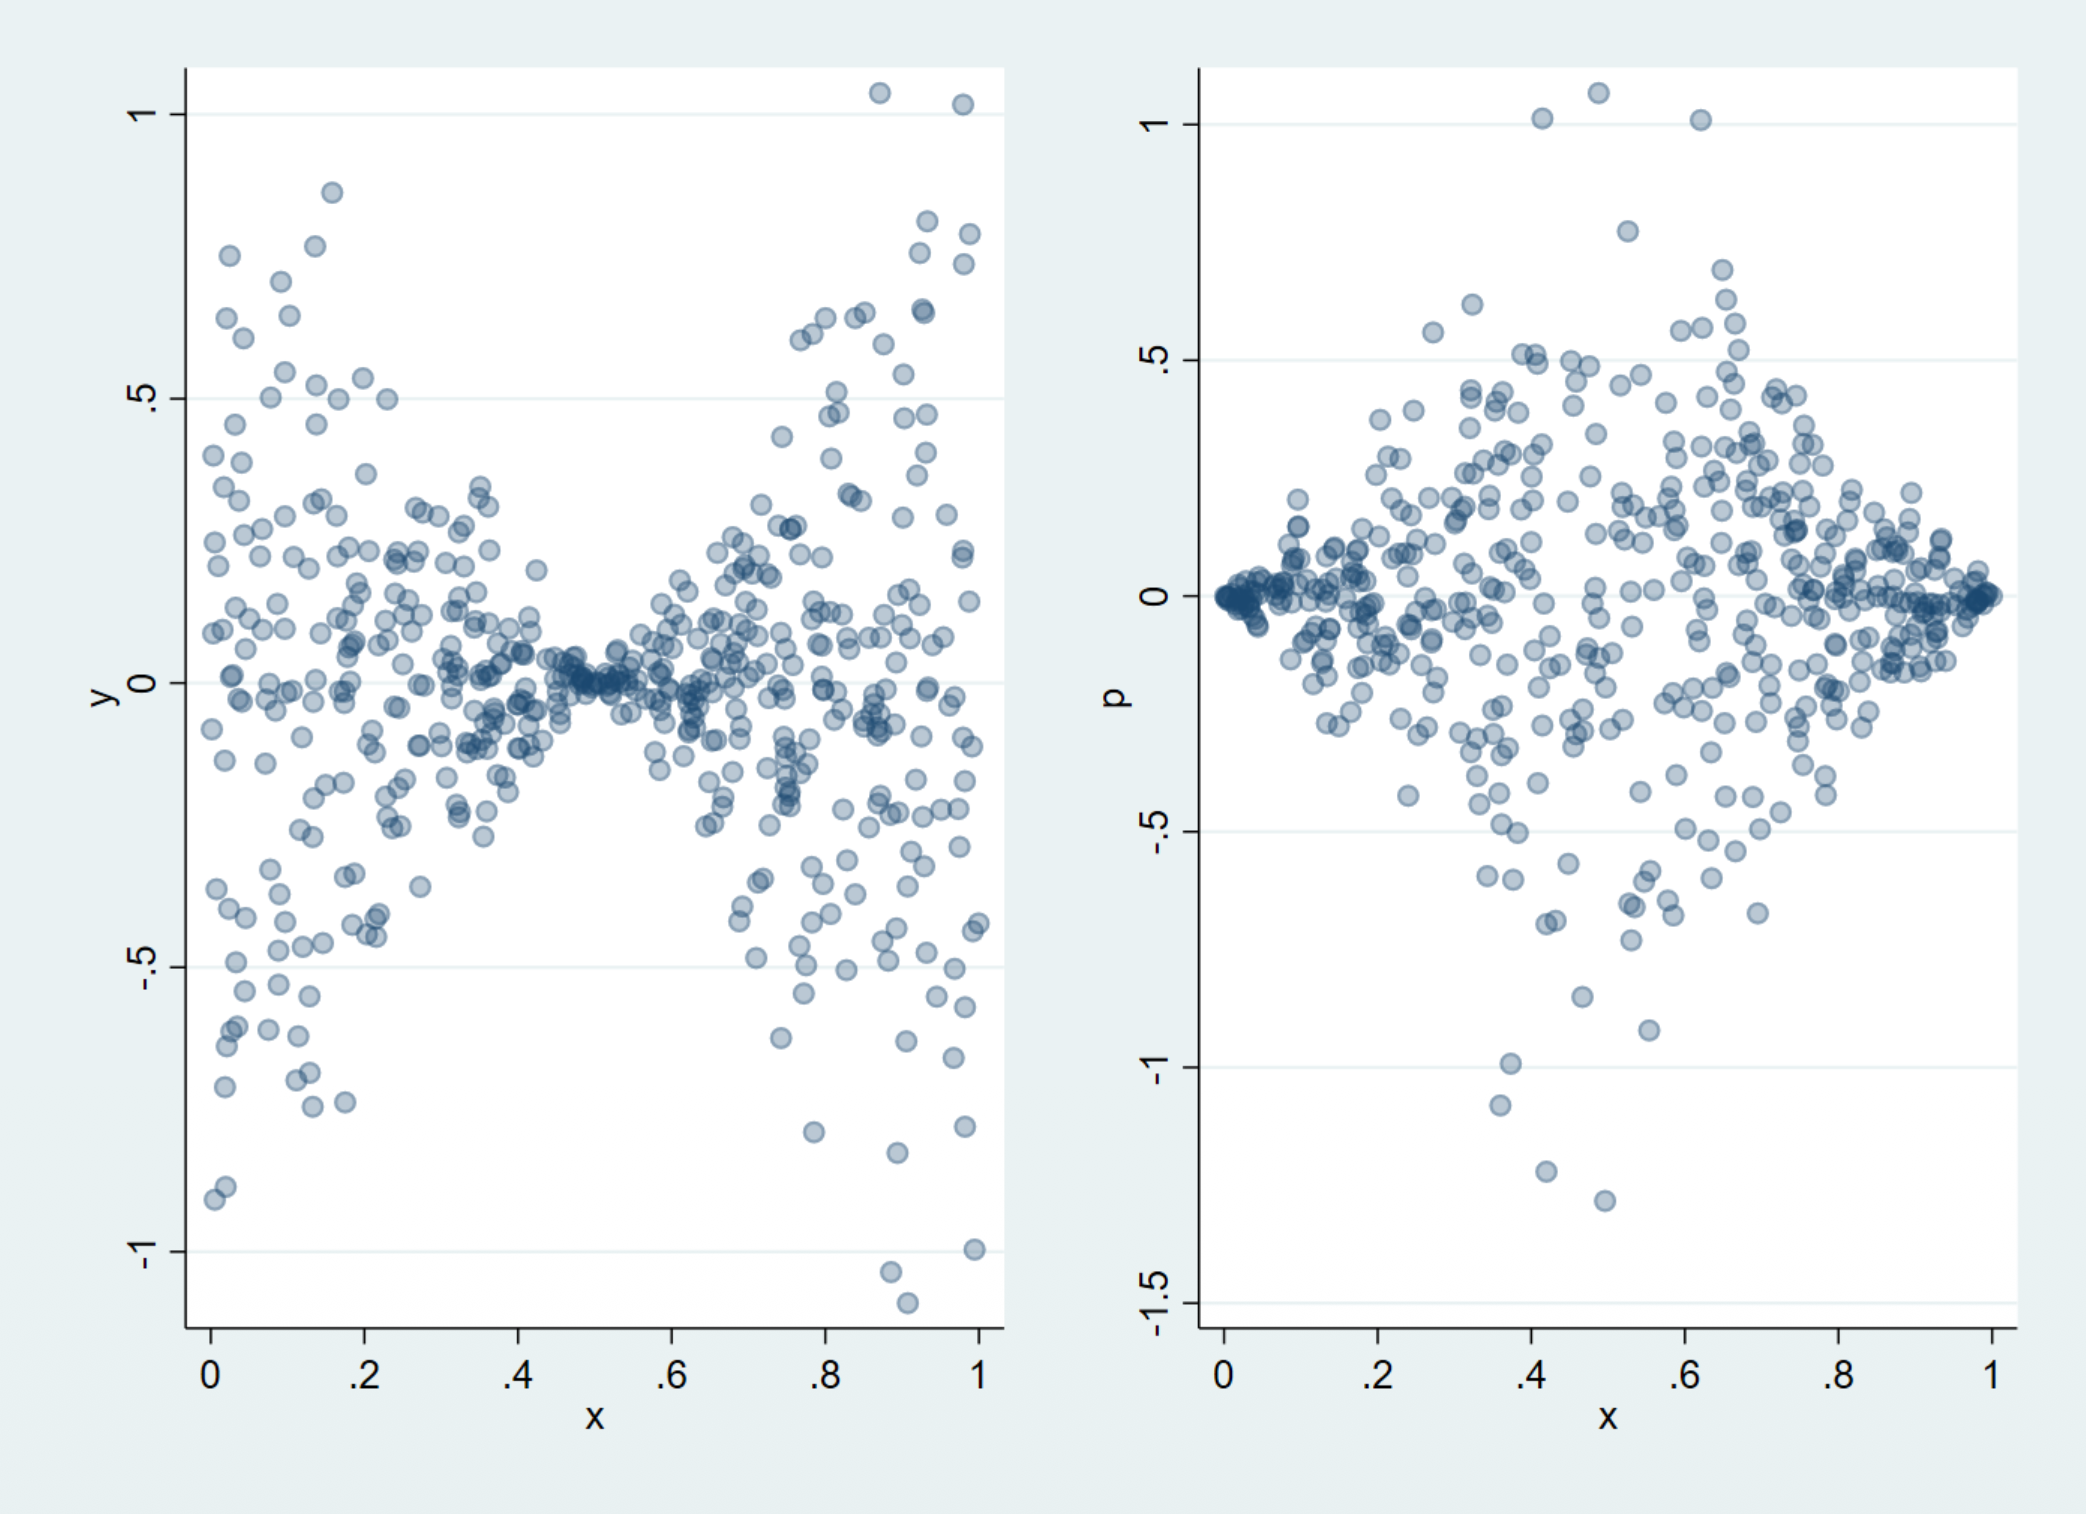
\includegraphics[width=0.78\textwidth]{images/2-12-1}
\end{figure}
Recalling a previous example, it should be much easier to estimate the slope $\beta_1$ from the data on the right, because the concentrations of mass are spread apart.
In fact, the heteroskedastic-robust standard error is smaller than the nonrobust standard error, so it is \emph{not} true that heteroskedastic-robust standard errors are always larger than nonrobust ones.

\begin{remark}	If MLR.5 holds: $\operatorname{Var}(u_i \mid x_i) = \sigma^2$. Since the error variance does not depend on the value of $x_i$, it is called homoskedastic.
	
	If the error variance depends on $x_i$, $u_i$ is heteroskedastic and MLR.5 fails.
	
	If MLR.1-4 are maintained, OLS is still unbiased and consistent under heteroskedasticity, but now the error variance depends on $x_i$: \[
		\operatorname{Var}(u_i \mid x_i) = \sigma_i^2
	,\] which in turn changes $\operatorname{Var}(\hat{\beta}_j \mid X)$.
\end{remark}

	\begin{remark}	If MLR.5 fails, and we use the wrong standard error, we may conclude that our result is significant because we mis-specified the variance of the estimator. This is why generalised least squares is not typically used and instead people do OLS with heteroskedasticity-robust standard errors (using the long form of asymptotic variance).

	Hence, while OLS will be unbiased and consistent, if we end up using the wrong test statistic in our hypothesis test, we may come to a wrong conclusion.

		We also note that using robust standard errors is valid when we have homoskedasticity, but we cannot use non-robust standard errors with heteroskedasticity. (Obviously, but we just need to emphasize this.) For example, consider the two regressions that use nonrobust and robust standard errors and the test statistic $\frac{\hat{\beta}_{\text{lotsize}}}{se\left( \hat{\beta}_{\text{lotsize}} \right)}$.
	\begin{figure}[htpb]
	  \centering
	  \begin{minipage}{0.49\textwidth}
	    \centering
	    \caption{Non-robust standard errors}
	    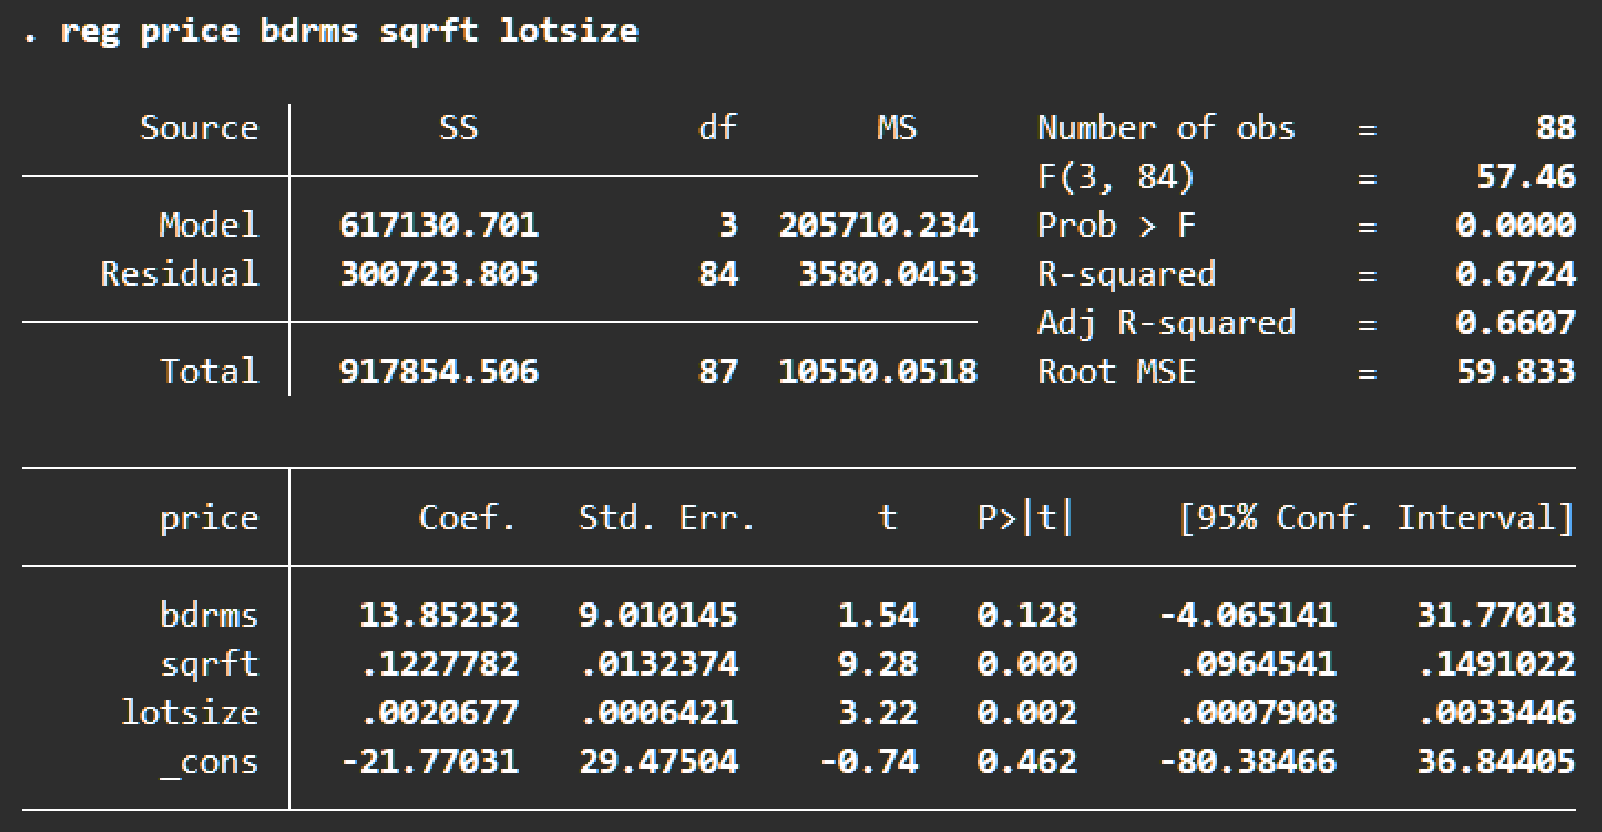
\includegraphics[width=\textwidth]{images/2-12-2}
	  \end{minipage}
	  \hfill
	  \begin{minipage}{0.49\textwidth}
	    \centering
	    \caption{Robust standard errors}
	    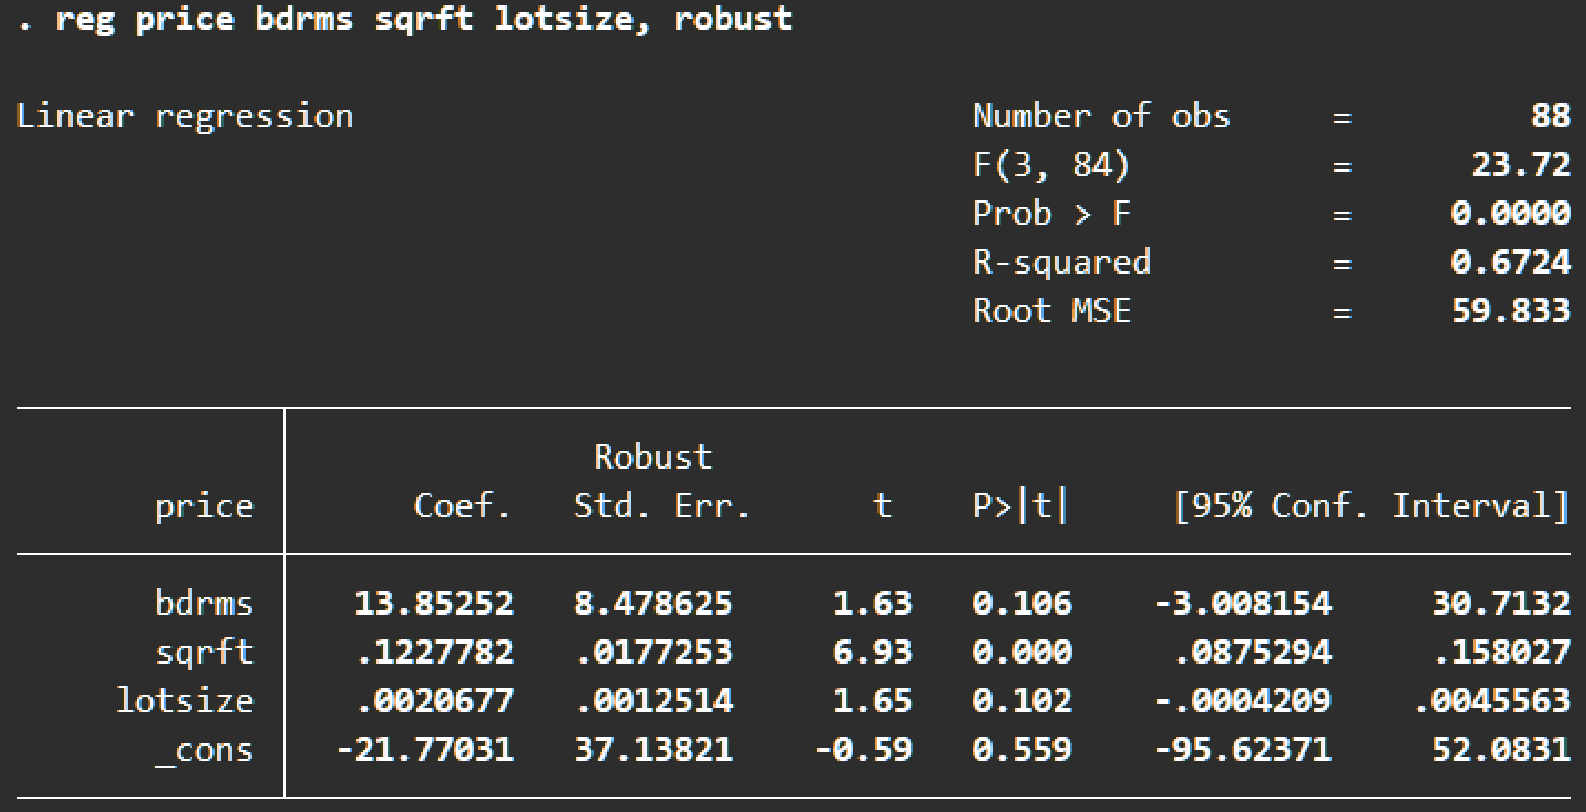
\includegraphics[width=\textwidth]{images/2-12-3}
	  \end{minipage}
	\end{figure}

	When would we ever use non-robust standard errors, then? 
	The advantage of non-robust standard errors is that $t$-stats have exact $t$-distributions under MLR.1-6.
	
	With robust standard errors, we need to use the approximation: \[
		\frac{\hat{\beta}_j - \beta_j}{\operatorname{se}_{\text{rob}}(\hat{\beta}_j)} \approx N(0,1)
	.\] 
	
	In practice, robust standard errors are used because they are valid with any form of heteroskedasticity, while justifying either of MLR.5 (homoskedasticity) or MLR.6 (normality of errors conditional on $X$) is difficult.
\end{remark}

	\begin{proposition}[Variance for individual coefficients]
		When $y_i = \beta_0 + \beta_1 x_{i1} + \cdots + \beta_k x_{ik} + u_i$, we find
		\begin{align*}
			\hat{\beta}_j = \left( X_j' M_{X_{-j}} X_j \right)^{-1} X_j' M_{X_{-j}} Y
		,\end{align*} so \[
			\hat{\beta}_j = \frac{\sum_{i=1}^{n} \hat{r}_{ij} y_i}{\sum_{i=1}^{n} \hat{r}_{ij}^2}
		,\] where $\hat{r}_{ij}$ denotes the $i$-th residual of a regression of $x_j$ on all other regressors.
	
	We find: \[
		\operatorname{Var}(\hat{\beta}_j \mid X) = \frac{\sum_{i=1}^{n} \hat{r}_{ij}^2 \operatorname{Var}(y_i \mid x_i)}{(\sum_{i=1}^{n} \hat{r}_{ij}^2)^2} = \frac{\sum_{i=1}^{n} \hat{r}_{ij}^2 \sigma_i^2}{(\sum_{i=1}^{n} \hat{r}_{ij}^2)^2}
	.\] 
	
	Because $\sigma_i^2$ is unknown, we replace it with $\E\left[u_i^2 \mid X_i\right] = \hat{u}_i^2$ and find: \[
		\widehat{\operatorname{Var}}(\hat{\beta}_j \mid X) = \frac{\sum_{i=1}^{n} \hat{r}_{ij}^2 \hat{u}_i^2}{(\sum_{i=1}^{n} \hat{r}_{ij}^2)^2}
	.\] 
	
	The heteroskedasticity robust standard error is given by\boxednote{Plugging $r_{i 1} = x_i - \overline{x}$ for a regression of $x_1$ onto a constant yields the expression we had in this section's exposition.} \[
		\operatorname{se}(\hat{\beta}_j) = \sqrt{\frac{\sum_{i=1}^{n} \hat{r}_{ij}^2 \hat{u}_i^2}{(\sum_{i=1}^{n} \hat{r}_{ij}^2)^2}}
	.\] 
\end{proposition}

\section{Weighted Least Squares}

\begin{proposition}[Weighted least squares transformation]
	If we knew the error variance $\sigma_i^2$, we could transform the model: \[
		\frac{y_i}{\sigma_i} = \left( \frac{1}{\sigma_i}, \frac{x_{i1}}{\sigma_i}, \ldots, \frac{x_{ik}}{\sigma_i} \right) \beta + \frac{u_i}{\sigma_i}
	.\] 

Notice that this model still satisfies MLR.4 since $\sigma_i$ only depends on $x_i$: \[
	\E\left( \frac{u_i}{\sigma_i} \mid x_i \right) = \frac{1}{\sigma_i} \E(u_i \mid x_i) = 0
.\] 

MLR.1-3 are unaffected, since multiplying each row of $X$ by a non-zero constant does not cause collinearity or change the interpretation of the model.

However, MLR.5 now holds, because \[
	\E\left[ \left( \frac{u_i}{\sigma_i} \right)^2 \mid \frac{x_i}{\sigma_i} \right] = \E\left[ \E\left[ \left( \frac{u_i}{\sigma_i} \right)^2 \mid x_i \right] \mid \frac{x_i}{\sigma_i} \right]
,\] and \[
	\E\left[ \left( \frac{u_i}{\sigma_i} \right)^2 \mid x_i \right] = \frac{1}{\sigma_i^2} \E(u_i^2 \mid x_i) = \frac{\sigma_i^2}{\sigma_i^2} = 1
.\] 

	OLS on the transformed model gives the best linear unbiased estimator of $\beta$ by the Gauss--Markov Theorem.\boxednote{There is some nuance here: Gauss--Markov gives us efficiency conditional on $\left(\frac{x_i}{\sigma_i}\right)$, but we will show in another problem set that it can be efficient conditional on $x$ as well.}
\end{proposition}

We really will just consider weighted least squares with homoskedasticity at the individual level. Geralized least squares weights based on the error variance, but this is beyond the scope of this course.

\begin{example}[WLS: Grouped Data]
	Suppose the model for observation $i$ is \[
		y_i = \beta_0 + \beta_1 x_i + u_i
	,\] where MLR.1-5 hold. Let $\operatorname{Var}(u \mid x) = \sigma^2$.
	
	Our observations are group averages e.g. mean age/income by zip code.
	
	There are $K$ groups $k = 1, \ldots, K$, and we observe \[
		\bar{y}_k = \frac{1}{n_k} \sum_{i \in \text{Group } k} y_i; \quad \bar{x}_k = \frac{1}{n_k} \sum_{i \in \text{Group } k} x_i
	\] for each $k = 1, \ldots, K$.
	
	We would actually run the regression on zip-code level data, so we make clear that the model written for averages is: \[
		\bar{y}_k = \beta_0 + \beta_1 \bar{x}_k + \bar{u}_k
	.\] 
	The error variance is \[
		\operatorname{Var}(\bar{u}_k \mid X) = \frac{\sigma^2}{n_k}
	.\] 
	This would actually give a different estimator of $\beta$ (since the weighting is uniform across zip codes, and not individuals as in the granular regression), and has heteroskedasticity.

	Hence, we should multiply by $\sqrt{n_k}$ to restore MLR.5\footnote{Note: we only recover homoskedasticity with this simple weighting because the original individual data was homoskedastic.} and estimate the following by OLS: \[
		\sqrt{n_k} \cdot \bar{y}_k = \beta_0 \cdot \sqrt{n_k} + \beta_1 \sqrt{n_k} \cdot \bar{x}_k + \sqrt{n_k} \cdot \bar{u}_k
	.\] 
	Here, $\operatorname{Var}(\sqrt{n_k} \cdot \bar{u}_k \mid X) = n_k \operatorname{Var}(\bar{u}_k \mid X) = \sigma^2$.
\end{example}

\section{Regression Specification}

\begin{remark}	Multiple linear regression can be used to model non-linear patterns in the data.
	
	We discuss:
	\begin{itemize}
		\item Using logarithms and polynomials to model non-linear patterns
		\item Turning continuous variables into qualitative variables
		\item Using qualitative variables to allow categories in the data to have their own coefficients
		\item Using interactions to allow the effect of changing one explanatory variable on the conditional mean to vary with the value of another.
	\end{itemize}
\end{remark}

\begin{remark}[Logarithms]
	Logarithms are often used to approximate proportional changes. For $x'$ close to $x$: \[
		\log(x') - \log(x) \approx \frac{x' - x}{x}
	\] by a first-order Taylor expansion, which is the proportional change from $x$ to $x'$.
	
	Several specifications used for conditional mean: \begin{align*}
		\E(y \mid x = t) &\approx \alpha + \beta \log(t) \quad \text{``level-log''} \\
		\E(\log(y) \mid x = t) &\approx \alpha + \beta t \quad \text{``log-level''} \\
		\E(\log(y) \mid x = t) &\approx \alpha + \beta \log(t) \quad \text{``log-log''}
	.\end{align*}
\end{remark}

Differentiating a conditional expectation is difficult, since we don't want to move the derivative operator in the expectation. Thus, the easiest log model to interpret is the log-level specification.

\begin{remark}[level-log specification]
	Consider $\E\left[y \mid x = t\right] = \alpha + \beta \ln{\left(t\right)}$.

	We have \begin{align*}
		\E(y \mid x = t + \Delta t) - \E(y \mid x = t) &\approx \beta[\log(t + \Delta t) - \log(t)] \\
		&\approx \beta \cdot \frac{\Delta t}{t} \\
		&= \frac{\beta}{100} \cdot \frac{100\Delta t}{t}
	,\end{align*} so $\beta/100$ is approximately the change in the conditional mean of $y$ when $t$ increases by $1\%$.\boxednote{This percentage interpretation is only valid for a causal interpretation, in that we examine a level of $t$ and error, then see the change in $y$ when increasing $t$. But we cannot differentiate a random variable with respect to another carelessly.}
\end{remark}

\begin{remark}[log-level specification]
	We have \[
		\E(\log(y) \mid x = t + 1) - \E(\log(y) \mid x = t) \approx \beta
	.\] 
	
		Expectations don't pass through non-linear functions (e.g. Jensen), but the following approximation leads to the common interpretation that a unit increase in $x$ is associated with a $\beta\%$ change in the mean of $y$:\boxednote{Jensen's inequality means $\E[\log y \mid x]$ need not equal $\log \E[y \mid x]$. The approximation is exact when $y \mid x$ is log-normal.} \begin{align*}
			\beta &\approx \E(\log(y) \mid x = t + 1) - \E(\log(y) \mid x = t) \\
			&\approx \log(\E(y \mid x = t + 1)) - \log(\E(y \mid x = t)) \\
			&\approx \frac{\E(y \mid x = t + 1) - \E(y \mid x = t)}{\E(y \mid x = t)}
	,\end{align*} so $100\beta$ is approximately the percentage change in the mean of $y$ resulting from a unit increase in $x$.
	
	Alternatively, exponentiating the first approximation and subtracting $1$ gives: \begin{align*}
		\exp(\beta) - 1 &\approx \exp(\E(\log(y) \mid x = t + 1) - \E(\log(y) \mid x = t)) - 1 \\
		&= \frac{\exp(\E(\log(y) \mid x = t + 1)) - \exp(\E(\log(y) \mid x = t))}{\exp(\E(\log(y) \mid x = t))}
	.\end{align*}
	Given that $\exp(x) \approx 1 + x$ when $x \approx 0$, the left hand side is approximately equal to $\beta$ if $\beta \approx 0$.
	
	We can therefore interpret $\beta$ as the proportional change in the conditional geometric mean of $y$ given a unit increase in $x$, holding the error term fixed.
\end{remark}

\begin{remark}[log-log specification]
	Now we have \[
		\E(\log(y) \mid x = t + \Delta t) - \E(\log(y) \mid x = t) \approx \beta[\log(t + \Delta t) - \log(t)]
	.\] 
	
	Combining the approximations for log-level and level-log gives: \[
		\frac{\E(y \mid x = t + \Delta t) - \E(y \mid x = t)}{\E(y \mid x = t)} \approx \beta \cdot \frac{\Delta t}{t}
	,\] so a $1\%$ increase in $t$ is associated with a $\beta\%$ change in the conditional mean of $y$ (also known as an elasticity).
\end{remark}

\begin{example}[Returns to experience]
	Consider the approximation: \[
		\E(\text{wage} \mid \text{exper}) \approx \beta_0 + \beta_1 \text{exper} + \beta_2 \text{exper}^2
	.\] 
	
	Experience estimated to have a diminishing marginal effect on wage.
	
	Turning point estimated where \[
		\frac{\partial \E(\text{wage} \mid \text{exper} = e^*)}{\partial e} = \hat{\beta}_1 + 2\hat{\beta}_2 e^* = 0 \implies e^* = -\frac{\hat{\beta}_1}{2\hat{\beta}_2} \approx 24
	.\] 
\end{example}

\begin{remark}[Returns to Experience]
	Issues with a causal interpretation:
	\begin{itemize}
		\item Omitted Variables Bias: Education impacts wage and may be correlated with/interact with exper or exper$^2$.
		\item Functional form misspecification: $w$ or $\ln(w)$? Quadratic in experience?
	\end{itemize}
	
	Average partial effect: What is the marginal effect of experience? \[
		\frac{\partial \E(\text{wage} \mid \text{exper} = e)}{\partial e} = \beta_1 + 2\beta_2 e
	.\] 
	The effect of experience diminishes if $\beta_2 < 0$. We can estimate the average partial effect: \[
		\widehat{\text{APE}} = \frac{1}{n} \sum_{i=1}^{n} (\hat{\beta}_1 + 2\hat{\beta}_2 \text{exper}_i) = \hat{\beta}_1 + 2\hat{\beta}_2 \overline{\text{exper}}_n
	.\] 
\end{remark}

\begin{remark}[Dummy Variables]
	Suppose we want to measure the difference in average wages between the tech industry and all other industries.
	
	Use a ``Dummy Variable'' to denote categories within data.
\end{remark}

\begin{remark}[Continuous variables to categorical variables]
	Suppose we are interested in estimating store sales by age category:
	\begin{itemize}
		\item Observe sales figures and age of customers.
		\item Create $k$ categories as follows: \[
			d_{i1} = \begin{cases}
				1 & \text{if } i \text{ is between 0-18 years of age} \\
				0 & \text{otherwise}
			\end{cases}
		\] \[
			d_{i2} = \begin{cases}
				1 & \text{if } i \text{ is between 18-25 years of age} \\
				0 & \text{otherwise}
			\end{cases}
		\] \[
			\vdots
		\] \[
			d_{ik} = \begin{cases}
				1 & \text{if } i \text{ is 75+ years of age} \\
				0 & \text{otherwise}
			\end{cases}
		\] 
	\end{itemize}
	
	Note: Groups are mutually exclusive ($d_{ij} d_{ik} = 0$ when $i \ne j$) and exhaustive ($d_{i1} + \cdots + d_{ik} = 1$).
	
	Means WLOG we can describe average sales by age category using \[
		\E(y_i \mid d_{i1}, \ldots, d_{ik}) = \beta_1 d_{i1} + \beta_2 d_{i2} + \cdots + \beta_k d_{ik}
	,\] where intercept is excluded to avoid perfect collinearity.
	
	Can also specify \[
		\E(y_i \mid d_{i1}, \ldots, d_{ik}) = \alpha_0 + \alpha_1 d_{i1} + \alpha_2 d_{i2} + \cdots + \alpha_{k-1} d_{ik-1}
	.\] 
	
	Note: \[
		\alpha_1 = \E(y \mid d_{i1} = 1, \ldots, d_{ik} = 0) - \E(y \mid d_{i1} = 0, \ldots, d_{ik} = 1)
	\] is interpreted as the difference in average spend between the youngest and oldest age categories.
	
	Excluding the dummy variable for the oldest category specifies that category as the base group.
	
	Intercept $\alpha_0$ is the mean for the base group.
	
	$\alpha_j$ represents difference in means between group $j$ and base group.
\end{remark}

\begin{remark}[Kinks and Jumps]
	Describe credit limits offered to new customers as a function of credit score.
	
	Sometimes outcome will change sharply at a cutoff. Suppose $y$ is credit limit and $x$ is credit score.
	
	Suppose only two categories of credit: 'Good' and 'Excellent'.
	
	Features:
	\begin{itemize}
		\item Sharp discontinuity in credit limit as soon as individual crosses 'Excellent' boundary
		\item Each additional unit of credit score improves credit limit more for individuals with excellent credit (Kink)
	\end{itemize}
	
	Let \[
		d_i = \begin{cases}
			1 & \text{if individual } x_i \ge 0.5 \\
			0 & \text{if individual } x_i < 0.5
		\end{cases}
	\] 
	
	Model: \begin{align*}
		y_i &= \beta_0 + \beta_1 x_i + d_i(\gamma + \delta x_i) + \epsilon_i \\
		&= \beta_0 + \beta_1 x_i + \gamma d_i + \delta d_i x_i + \epsilon_i
	.\end{align*}
	
	When $x_i < a$: $\E(y_i \mid x = x_i) = \beta_0 + \beta_1 x_i$.
	
	When $x_i \ge a$: $\E(y_i \mid x = x_i) = (\beta_0 + \gamma) + (\beta_1 + \delta) x_i$.
	
	Note: not all parameters have a useful interpretation: $\beta_0 + \gamma$ is the credit limit an individual with 'Excellent' credit would receive if their credit score were $0$ (We could never observe such individuals in the data).
	
	$\delta$ represents the additional return to credit score for individuals with excellent credit.
	
	Jump: $\gamma + \delta \cdot 0.5$.
\end{remark}

\begin{remark}[Saturated Regression]
	Describe wages in tech vs. not in tech, both inside and outside california: \[
		\E(W \mid T, C) = \beta_0 + \beta_1 T + \beta_2 C + \beta_3 T \cdot C
	.\] 
	We call this a saturated regression since it has one parameter for each possible value of the regressors: \[
		(T, C) \in \{(0,0), (1,0), (0,1), (1,1)\}
	.\] 
	
	The equality holds by construction, not because of an additional assumption about linearity of the conditional mean.
	
	Could also specify \[
		\E(W \mid T, C) = \alpha_0 (1-T) \cdot (1-C) + \alpha_1 T \cdot (1-C) + \alpha_2 (1-T) \cdot C + \alpha_3 T \cdot C
	.\] 
	
	Only difference is in interpretation of parameters: \begin{align*}
		\E(W \mid T = 0, C = 0) &= \beta_0 = \alpha_0 \\
		\E(W \mid T = 1, C = 0) &= \beta_0 + \beta_1 = \alpha_1 \\
		\E(W \mid T = 0, C = 1) &= \beta_0 + \beta_2 = \alpha_2 \\
		\E(W \mid T = 1, C = 1) &= \beta_0 + \beta_1 + \beta_2 + \beta_3 = \alpha_3
	.\end{align*}
	
	$\beta_1$ represents difference in average wages in tech vs. not for employees outside california.
	
	$\beta_2$ represents difference in average wages in california vs. not for employees not in tech.
	
	$\beta_3$ represents a ``difference in differences''. For example: \begin{align*}
		\beta_3 &= [(\beta_0 + \beta_1 + \beta_2 + \beta_3) - (\beta_0 + \beta_2)] - [(\beta_0 + \beta_1) - \beta_0] \\
		&= [\E(W \mid T = 1, C = 1) - \E(W \mid T = 0, C = 1)] \\
		&\quad - [\E(W \mid T = 1, C = 0) - \E(W \mid T = 0, C = 0)]
	.\end{align*}
	
	This is the difference (between california and not) in differences in wages inside and outside tech.
\end{remark}

	\begin{remark}[Interactions]
		An interaction is a product of two regressors. e.g. \[
			\text{wage} = \beta_0 + \beta_1 \text{educ} + \beta_2 \text{exper} + \beta_3 \text{educ} \cdot \text{exper} + \epsilon
	.\] 
	
		If $\E(\epsilon \mid \text{educ}, \text{exper}) = 0$, we have: \[
			\frac{\partial}{\partial \text{exper}} \E(\text{wage} \mid \text{educ}, \text{exper}) = \beta_2 + \beta_3 \text{educ}
		,\] so if $\beta_3 > 0$, average wage for those with more education differs more across experience levels.
	\end{remark}

\section{Summary}

\begin{remark}[Model and estimator]
	\leavevmode\hfill\break
	\textbf{Model}: $y = x'\beta + u$ with $\E\left[xu\right] = 0$. \\
	\textbf{Estimator}: $\hat{\beta}^{OLS} = (X'X)^{-1}X'Y$. \\
	\textbf{Interpretation}: each coefficient is the slope of the conditional mean with the remaining regressors held fixed.
\end{remark}

\begin{remark}[Finite-sample inference under normality]
	Suppose $Y \mid X \sim N(X\beta,\sigma^2 I_n)$. Exact conditional distributions:
	\[
		\begin{aligned}
			\hat{\beta} \mid X &\sim N\left(\beta,\sigma^2 (X'X)^{-1}\right), \\
			\hat{\sigma}^2 = \frac{SSR}{n-k} &\sim \frac{\sigma^2}{n-k}\chi^2_{n-k}
		\end{aligned}
	.\]
	The key finite-sample fact is that $\hat{\beta}-\beta$ and $\hat{\sigma}^2$ are conditionally independent, which yields exact $t_{n-k}$ tests and confidence intervals.
\end{remark}

\begin{remark}[Large-sample inference]
	Without normality, asymptotic normality replaces exact finite-sample formulas:
	\[
		\sqrt{n}(\hat{\beta}_n-\beta) \xrightarrow{d} N(0,V)
	.\]
	Single restrictions use asymptotic $z$-tests and confidence intervals, while multiple restrictions use $\chi^2_p$ statistics and ellipsoidal confidence sets for $R\beta$.
\end{remark}

\begin{remark}[Homoskedastic vs.\ heteroskedastic inference]
		\begin{center}
		\small
		\renewcommand{\arraystretch}{1.1}
		\begin{tabular}{p{0.20\linewidth}p{0.27\linewidth}p{0.33\linewidth}}
			\toprule
			Case & Standard error formula & Inference to use \\
			\midrule
			Homoskedastic, normal & $\hat{\sigma}^2(X'X)^{-1}$ & Exact $t$ / exact finite-sample \\
			Homoskedastic, large sample & $\hat{\sigma}^2(X'X)^{-1}$ & Asymptotic normal / $\chi^2$ \\
			Heteroskedastic & $(X'X)^{-1}X'\hat{\Omega}X(X'X)^{-1}$ & Robust asymptotic normal / $\chi^2$ \\
			\bottomrule
		\end{tabular}
		\end{center}
		Robust standard errors are valid in both homoskedastic and heteroskedastic settings, but exact $t$ inference requires the stronger homoskedastic-normal setup.
\end{remark}

\begin{remark}[Weighted least squares]
	If $\operatorname{Var}(u_i \mid x_i) = \sigma_i^2$ is known, divide the $i$-th observation by $\sigma_i$ to restore homoskedasticity. OLS on the transformed model is WLS and is efficient within the class of linear unbiased estimators under the transformed homoskedastic model.
\end{remark}

\begin{remark}[Regression specifications]
	Common specifications and their interpretation:
	\begin{itemize}
		\item \textbf{Level-log}: $\beta/100$ is the change in $\E(y \mid x)$ for a $1\%$ increase in $x$.
		\item \textbf{Log-level}: $100\beta$ approximates the percent change in $\E(y \mid x)$ for a one-unit increase in $x$.
		\item \textbf{Log-log}: $\beta$ is an elasticity.
		\item \textbf{Dummies/interactions}: allow group-specific intercepts, slopes, and difference-in-differences style comparisons.
	\end{itemize}
\end{remark}
